\documentclass[oneside,a4paper,14pt]{extarticle}
\usepackage[a4paper,top=20mm,bottom=20mm,left=30mm,right=10mm]{geometry}
\usepackage{amsmath, amssymb, amsfonts, amsthm}
\usepackage[T2A]{fontenc}
\usepackage[utf8]{inputenc}
\usepackage[russian]{babel}
\usepackage{textcomp}
\usepackage{indentfirst}
\usepackage{graphicx}
\usepackage{float}
\usepackage{wrapfig}
\usepackage{caption}
\usepackage{tocloft}
\renewcommand{\cftsecleader}{\cftdotfill{\cftdotsep}}
\usepackage[breaklinks]{hyperref}
\usepackage{titlesec}
\usepackage{fancyvrb}
\usepackage{xcolor}
\titleformat{\section}{\normalsize\bfseries}{\thesection}{1em}{}
\titleformat{\subsection}{\normalsize\bfseries}{\thesubsection}{1em}{}
\titleformat{\subsubsection}{\normalsize\bfseries}{\thesubsubsection}{1em}{}
\renewcommand\baselinestretch{1.33}\normalsize
\setlength{\parindent}{1.25cm}

\begin{document}
\newpage\thispagestyle{empty}
\newpage
\setcounter{page}{1}
\tableofcontents
\newpage

\section*{Задание}
\addcontentsline{toc}{section}{Задание}
Задание для шестого варианта:\\
«Сдвигатель» 8-разрядного двоичного числа, содержащего в старшем (седьмом) разряде знак числа, на N $\le$ 7 разрядов в сторону младших разрядов (сдвиг арифметический)

\section*{Анализ задания по разработке функциональной модели}
\addcontentsline{toc}{section}{Анализ задания по разработке функциональной модели}

Разработать функциональную модель двоичного сдвигателя.\\

На первый вход подаётся 8-разрядный двоичный код\\$X=x_0,x_1,x_2,x_3,x_4,x_5,x_6,x_7$,
а на второй вход 3-разрядный двоичный код переноса $E=e_0,e_1,e_2$.\\

При $e_0,e_1,e_2=0$ на информационный выход $Y=y_0,y_1,y_2,y_3,y_4,y_5,y_6,y_7$ код поступает без изменений.\\

При $x_0=1,x_1=0,x_2=1,x_3=0,x_4=0,x_5=1,x_6=0,x_7=0$ (10100100) $e_2=1$ на информационном выходе формируется сдвинутый вправо на 1 бит 8-разрядный двоичный код:\\
$y_0=1,y_1=1,y_2=0,y_3=1,y_4=0,y_5=0,y_6=1,y_7=0$\\
(11010010)

При этом выход $y_7$ всегда будет равен $x_7$ и будет определять бит, которым будут заменяться младшие разряды.

\newpage
\section*{Описание работы узла с помощью системы булевых функций}
\addcontentsline{toc}{section}{Описание работы узла с помощью системы булевых функций}
Работа 8-разрядного узла сдвига может быть описана следующей системой булевых функций:\\

\begin{small}

$y_0=(x_0 \lor e_2 \lor e_1 \lor e_0) \land (x_1 \lor e_2 \lor e_1 \lor \lnot e_0) \land (x_2 \lor e_2 \lor \lnot e_1 \lor e_0) \land (x_4 \lor \lnot e_2 \lor e_1 \lor e_0) \land (x_7 \lor \lnot e_2 \lor \lnot e_1 \lor \lnot e_0) \land (x_3 \lor e_2 \lor \lnot e_1 \lor \lnot e_0) \land (x_5 \lor \lnot e_2 \lor e_1 \lor \lnot e_0) \land (x_6 \lor \lnot e_2 \lor \lnot e_1 \lor e_0)$\\

$y_1=(x_7 \lor \lnot e_2 \lor \lnot e_1) \land (x_1 \lor e_2 \lor e_1 \lor e_0) \land (x_2 \lor e_2 \lor e_1 \lor \lnot e_0) \land (x_4 \lor e_2 \lor \lnot e_1 \lor \lnot e_0) \land (x_3 \lor e_2 \lor \lnot e_1 \lor e_0) \land (x_6 \lor \lnot e_2 \lor e_1 \lor \lnot e_0) \land (x_5 \lor \lnot e_2 \lor e_1 \lor e_0)$\\

$y_2=(x_7 \lor \lnot e_2 \lor \lnot e_0) \land (x_7 \lor \lnot e_2 \lor \lnot e_1) \land (x_2 \lor e_2 \lor e_1 \lor e_0) \land (x_6 \lor \lnot e_2 \lor e_1 \lor e_0) \land (x_5 \lor e_2 \lor \lnot e_1 \lor \lnot e_0) \land (x_3 \lor e_2 \lor e_1 \lor \lnot e_0) \land (x_4 \lor e_2 \lor \lnot e_1 \lor e_0)$\\

$y_3=(x_7 \lor \lnot e_2) \land (x_3 \lor e_2 \lor e_1 \lor e_0) \land (x_6 \lor e_2 \lor \lnot e_1 \lor \lnot e_0) \land (x_4 \lor e_2 \lor e_1 \lor \lnot e_0) \land (x_5 \lor e_2 \lor \lnot e_1 \lor e_0)$\\

$y_4=(x_7 \lor \lnot e_2) \land (x_7 \lor \lnot e_1 \lor \lnot e_0) \land (x_5 \lor e_2 \lor e_1 \lor \lnot e_0) \land (x_6 \lor e_2 \lor \lnot e_1 \lor e_0) \land (x_4 \lor e_2 \lor e_1 \lor e_0)$\\

$y_5=(x_7 \lor \lnot e_1) \land (x_7 \lor \lnot e_2) \land (x_6 \lor e_2 \lor e_1 \lor \lnot e_0) \land (x_5 \lor e_2 \lor e_1 \lor e_0)$\\

$y_6=(x_7 \lor \lnot e_0) \land (x_7 \lor \lnot e_1) \land (x_7 \lor \lnot e_2) \land (x_6 \lor e_2 \lor e_1 \lor e_0)$\\

$y_7=x_7$\\

\end{small}

\section*{Разработка функциональной схемы узла}
\addcontentsline{toc}{section}{Разработка функциональной схемы узла}
На основе системы булевых функций, описывающей работу узла, может быть построена его функциональная схема. Функциональная схема узла инкремента изображена на рис. 1.

\begin{figure}[H]
    \centering
    \includegraphics[width=0.6\textwidth]{Сдвигатель.png}
    \caption{функциональная схема узла}
    \label{fig:form}
\end{figure}

\twocolumn
\section*{Представления MS Excel}
\addcontentsline{toc}{section}{представления MS Excel}

$y_7=B15$\\

$y_6$=IF(AND(\\
IF(OR(B15;P28));\\
IF(OR(B15;O26));\\
IF(OR(B15;N23));\\
IF(OR(C15;K15;L15;M15)));\\
1;0)\\

$y_5$=IF(AND(\\
IF(OR(B15;N23));\\
IF(OR(B15;O26));\\
IF(OR(C15;K15;L15;P28));\\
IF(OR(D15;K15;L15;M15)));\\
1;0)\\

$y_4$=IF(AND(\\
IF(OR(B15;N23));\\
IF(OR(B15;N23;P28));\\
IF(OR(D15;K15;L15;;P28));\\
IF(OR(C15;K15;M15;O26));\\
IF(OR(E15;K15;L15;M15)));\\
1;0)\\

$y_3$=IF(AND(\\
IF(OR(B15;N23));\\
IF(OR(F15;K15;L15;M15));\\
IF(OR(C15;K15;O26;P28));\\
IF(OR(E15;K15;L15;P28));\\
IF(OR(D15;K15;O26;M15)));\\
1;0)\\

$y_2$=IF(AND(\\
IF(OR(B15;N23;P28));\\
IF(OR(B15;N23;O26));\\
IF(OR(G15;K15;L15;M15));\\
IF(OR(C15;N23;L15;M15));\\
IF(OR(D15;K15;O26;P28));\\
IF(OR(F15;K15;L15;P28));\\
IF(OR(E15;K15;O26;M15)));\\
1;0)\\

$y_1$=IF(AND(\\
IF(OR(B15;N23;O26));\\
IF(OR(H15;K15;L15;M15));\\
IF(OR(G15;K15;L15;P28));\\
IF(OR(E15;K15;O26;P28));\\
IF(OR(F15;K15;M15;O26));\\
IF(OR(C15;N23;L15;P28));\\
IF(OR(D15;N23;L15;M15)));\\
1;0)\\

$y_0$=IF(AND(\\
IF(OR(I15;K15;L15;M15));\\
IF(OR(H15;K15;P28;L15));\\
IF(OR(G15;K15;M15;O26));\\
IF(OR(E15;N23;L15;M15));\\
IF(OR(B15;N23;O26;P28));\\
IF(OR(F15;K15;O26;P28));\\
IF(OR(D15;N23;L15;P28));\\
IF(OR(C15;N23;O26;M15)));\\
1;0)\\
\onecolumn

\section*{Разработка экранной формы для экспериментального исследования узла}
\addcontentsline{toc}{section}{Разработка экранной формы для экспериментального исследования узла}
Работа узла моделируется путем реализации формул булевых функций с помощью логических функций табличного процессора MS Excel.\\
На форме имеются поля для ввода разряда числа и переноса, вывода разрядов двоичного кода.На экран также выводятся инвертированные разряды значения переноса, значения каждого логического элемента.

\begin{figure}[H]
    \centering
    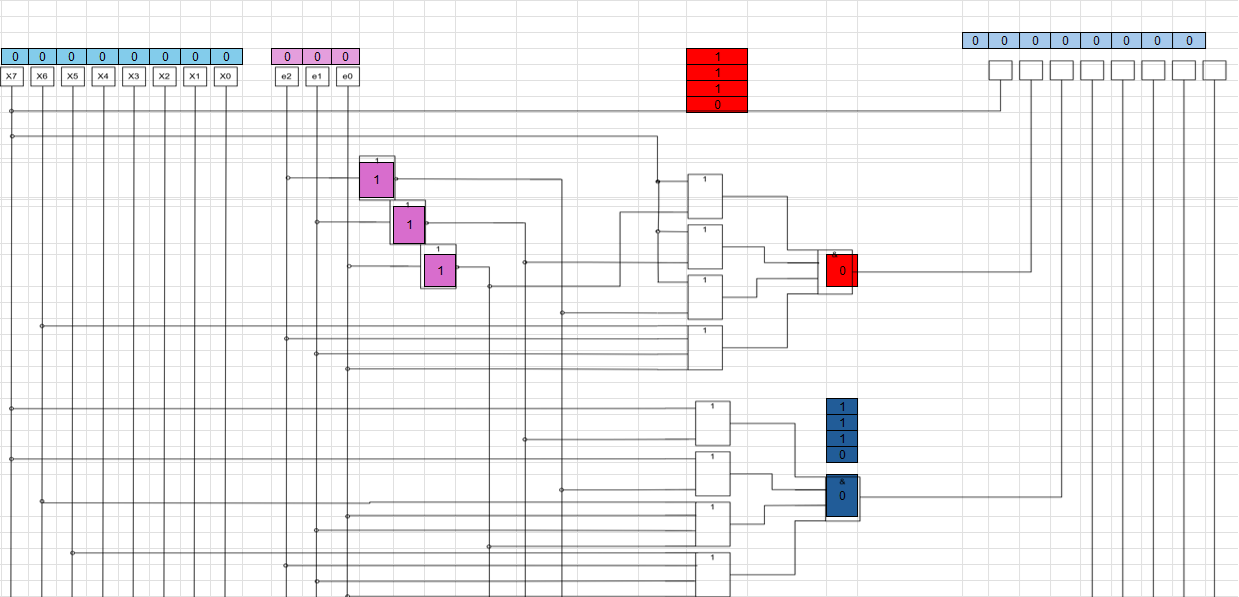
\includegraphics[width=0.9\textwidth]{1.png}
    \caption{экранная форма часть 1}
    \label{fig:exN1}
\end{figure}
\begin{figure}[H]
    \centering
    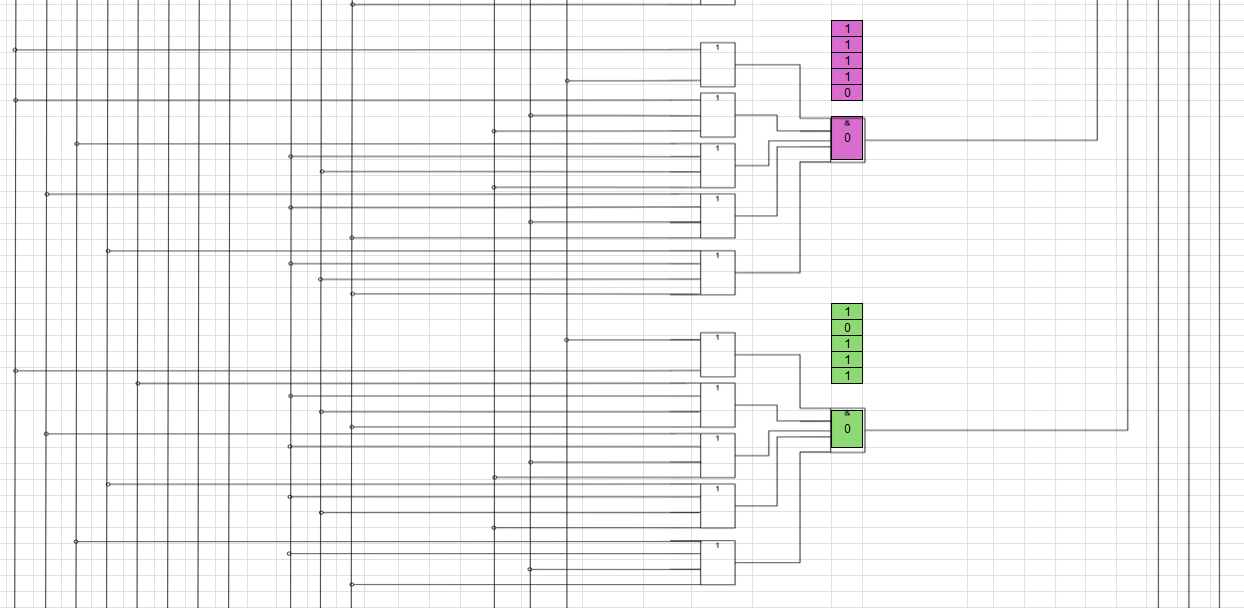
\includegraphics[width=1.0\textwidth]{2.png}
    \caption{экранная форма часть 2}
    \label{fig:exN2}
\end{figure}
\begin{figure}[H]
    \centering
    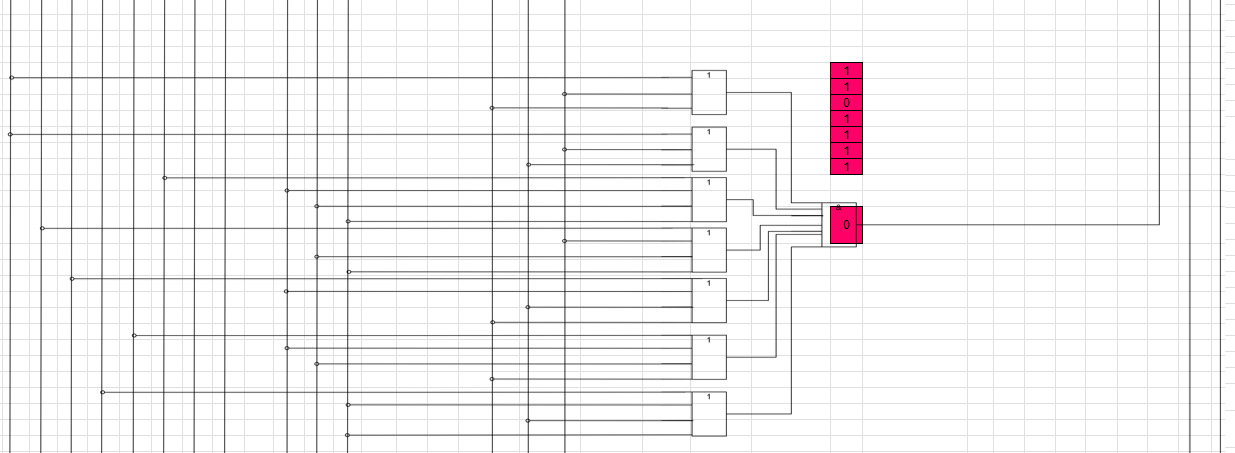
\includegraphics[width=1.0\textwidth]{3.png}
    \caption{экранная форма часть 3}
    \label{fig:exN3}
\end{figure}
\begin{figure}[H]
    \centering
    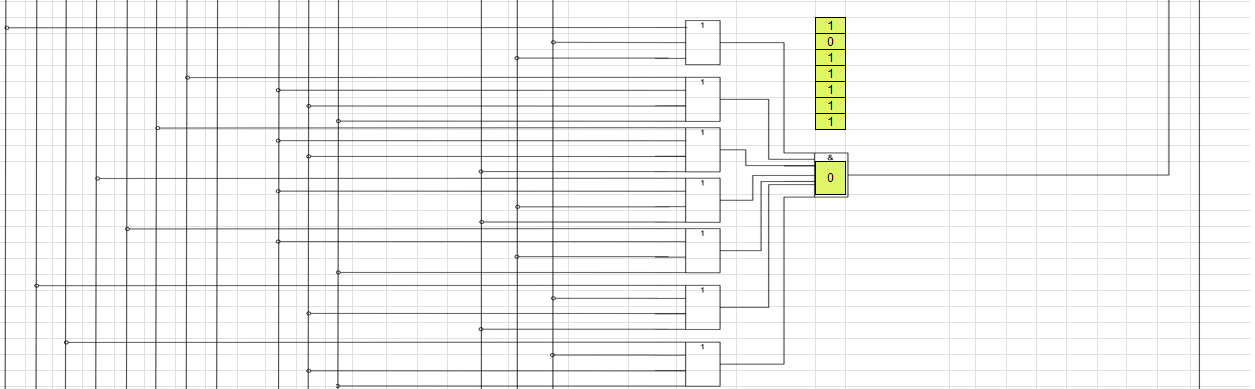
\includegraphics[width=1.0\textwidth]{4.png}
    \caption{экранная форма часть 4}
    \label{fig:exN4}
\end{figure}
\begin{figure}[H]
    \centering
    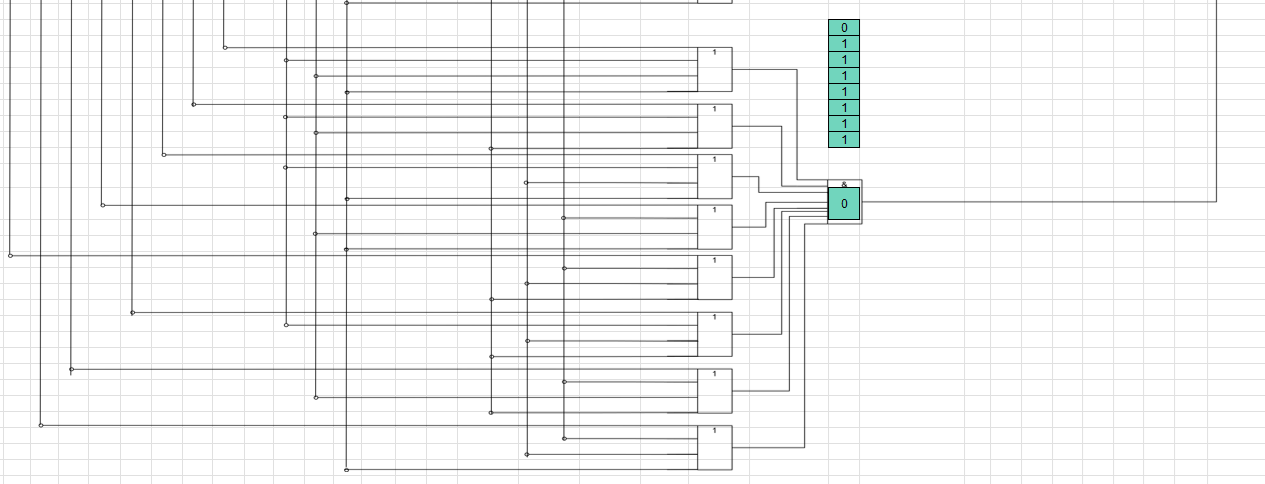
\includegraphics[width=1.0\textwidth]{5.png}
    \caption{экранная форма часть 5}
    \label{fig:exN5}
\end{figure}

\section*{Экспериментальные исследования функциональной модели узла}
\addcontentsline{toc}{section}{Экспериментальные исследования функциональной модели узла}
В процессе экспериментального исследования функциональной модели узла проверка правильности работы проводилась путём частичного перебора сочетаний значений входных переменных и сравнения соответствующих им выходных значений, со значениями полученными экспериментальным путём.\\
Результаты экспериментального исследования функциональной модели узла представлены в табл. 1.\\
\begin{small}

\begin{tabular}{|c|c|c|c|c|c|c|c|c|c|c|c|c|c|c|c|c|c|c|}
\hline
{$e_2$} & {$e_1$} & {$e_0$} &
{$x_7$} & {$x_6$} & {$x_5$} &
{$x_4$} & {$x_3$} & {$x_2$} &
{$x_1$} & {$x_0$} &
{$y_7$} & {$y_6$} & {$y_5$} &
{$y_4$} & {$y_3$} & {$y_2$} &
{$y_1$} & {$y_0$} \\
\hline
0 & 0 & 1 & 0 & 0 & 0 & 1 & 0 & 1 & 0 & 1 & 0 & 0 & 0 & 0 & 1 & 0 & 1 & 0 \\
\hline
0 & 0 & 1 & 0 & 1 & 0 & 0 & 1 & 0 & 0 & 1 & 0 & 0 & 1 & 0 & 0 & 1 & 0 & 0 \\
\hline
0 & 0 & 1 & 1 & 0 & 0 & 1 & 1 & 0 & 1 & 1 & 1 & 1 & 0 & 0 & 1 & 1 & 0 & 1 \\
\hline
0 & 1 & 0 & 1 & 1 & 0 & 1 & 0 & 0 & 0 & 0 & 1 & 1 & 1 & 1 & 0 & 1 & 0 & 0 \\
\hline
0 & 1 & 0 & 1 & 0 & 0 & 0 & 0 & 1 & 1 & 0 & 1 & 1 & 1 & 0 & 0 & 0 & 0 & 1 \\
\hline
0 & 0 & 1 & 1 & 0 & 1 & 1 & 0 & 0 & 1 & 1 & 1 & 1 & 0 & 1 & 1 & 0 & 0 & 1 \\
\hline
0 & 1 & 1 & 1 & 1 & 0 & 0 & 0 & 0 & 1 & 0 & 1 & 1 & 1 & 1 & 1 & 0 & 0 & 0 \\
\hline
\end{tabular}

\end{small}

\section*{Вывод}
\addcontentsline{toc}{section}{Вывод}
В ходе выполнения лабораторной работы была разработана схема булевых функций, описывающая работу сдвигателя. На основе схемы булевых функций были составлены их представления и составлена экранная форма узла для экспериментального исследования инструментами табличного процессора MS Excel. В ходе экспериментального исследования составлена таблица результатов, которая отражает работу узла без ошибок.

\end{document}